\begin{figure}[h!]
  \centering
  \begin{subfigure}[b]{0.2\linewidth}
    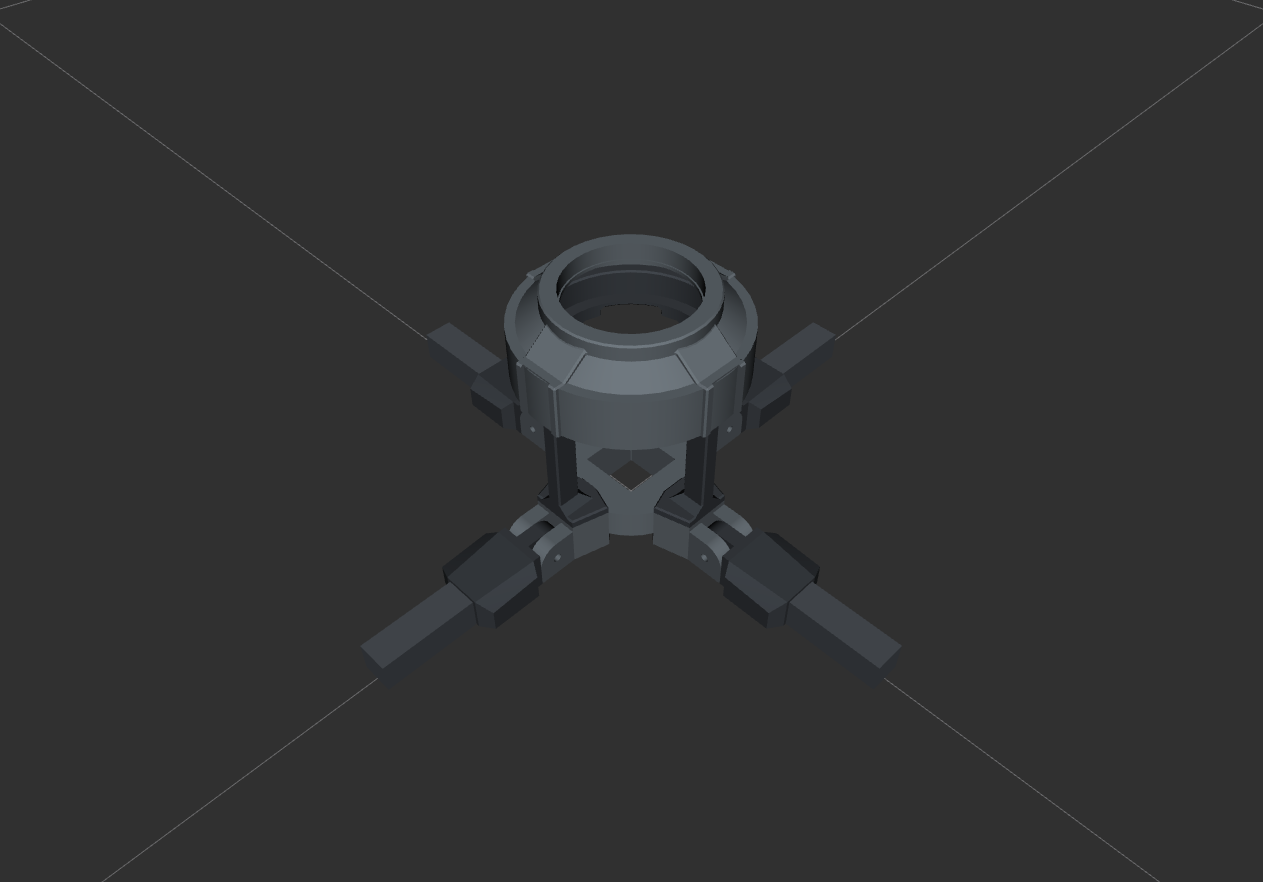
\includegraphics[width=\linewidth]{base.png}
     \caption{base link}
  \end{subfigure}
  \begin{subfigure}[b]{0.2\linewidth}
    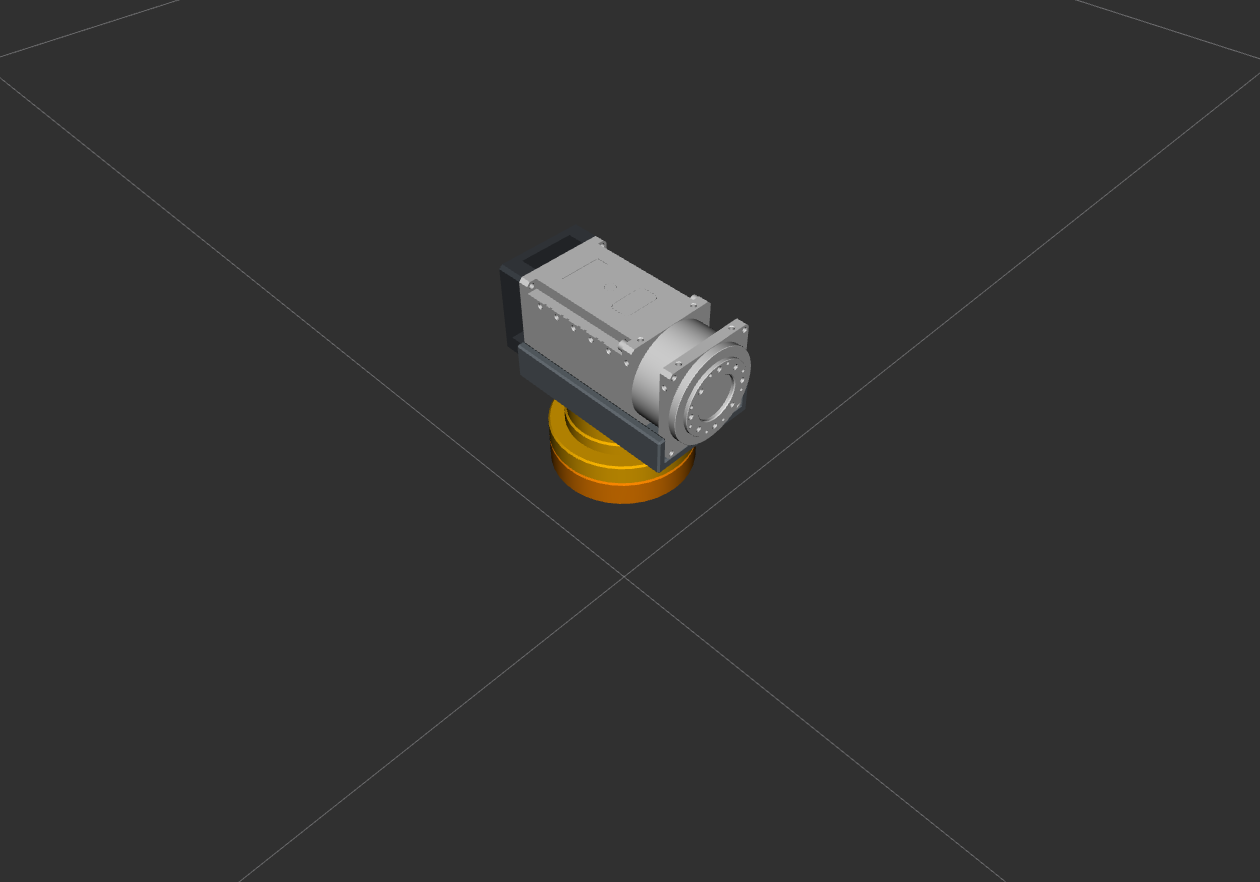
\includegraphics[width=\linewidth]{link1.png}
    \caption{link1}
  \end{subfigure}
  \begin{subfigure}[b]{0.2\linewidth}
    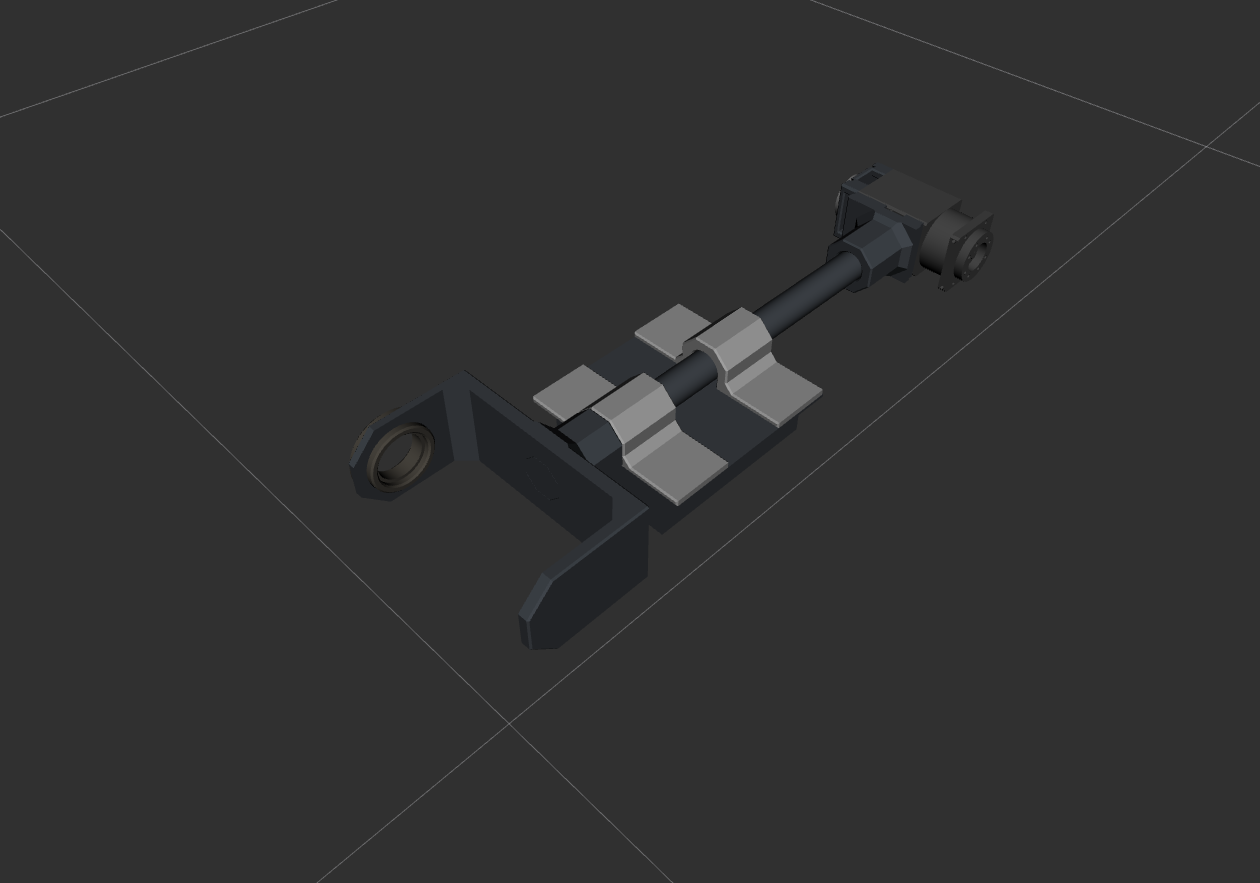
\includegraphics[width=\linewidth]{link2.png}
    \caption{link2}
  \end{subfigure}
  \begin{subfigure}[b]{0.2\linewidth}
    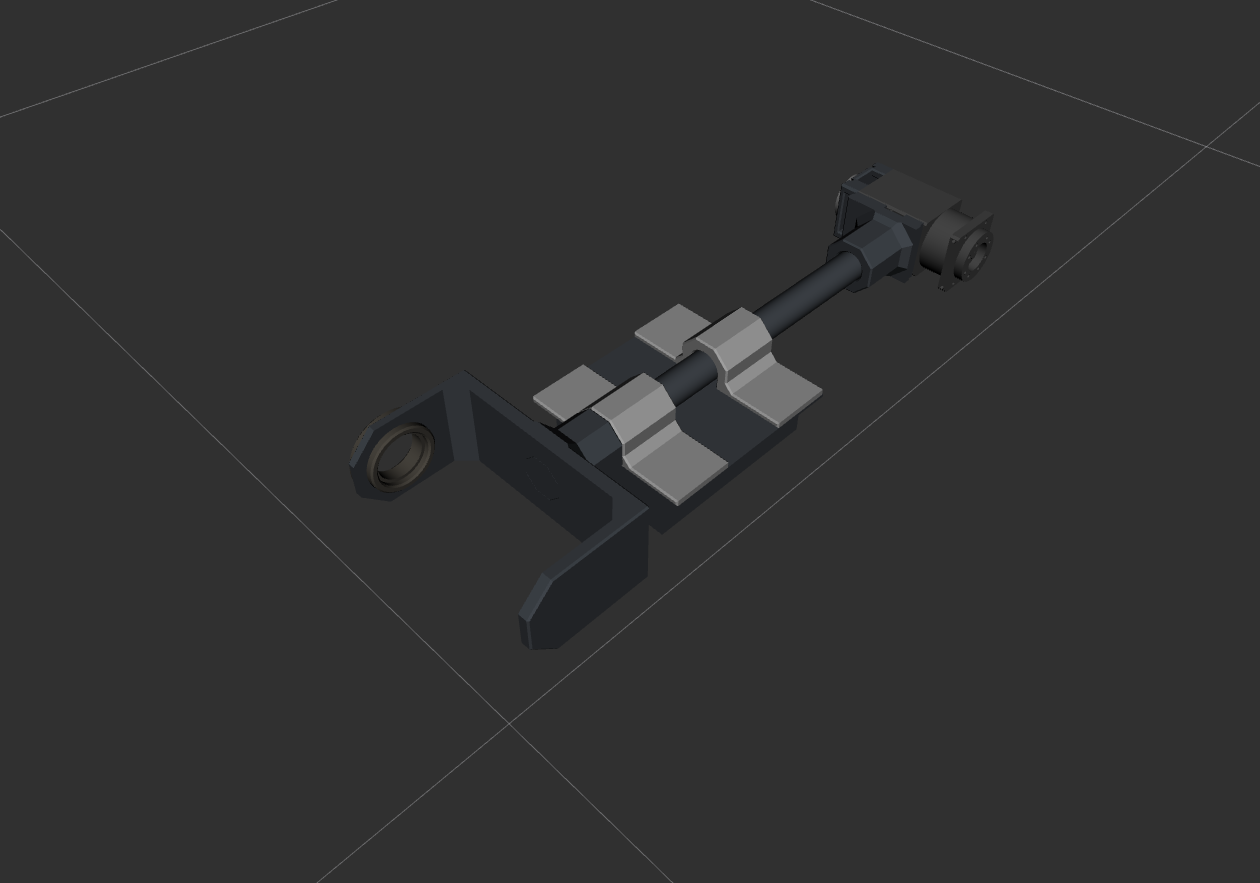
\includegraphics[width=\linewidth]{link2.png}
    \caption{link2}
  \end{subfigure}
  \begin{subfigure}[b]{0.2\linewidth}
    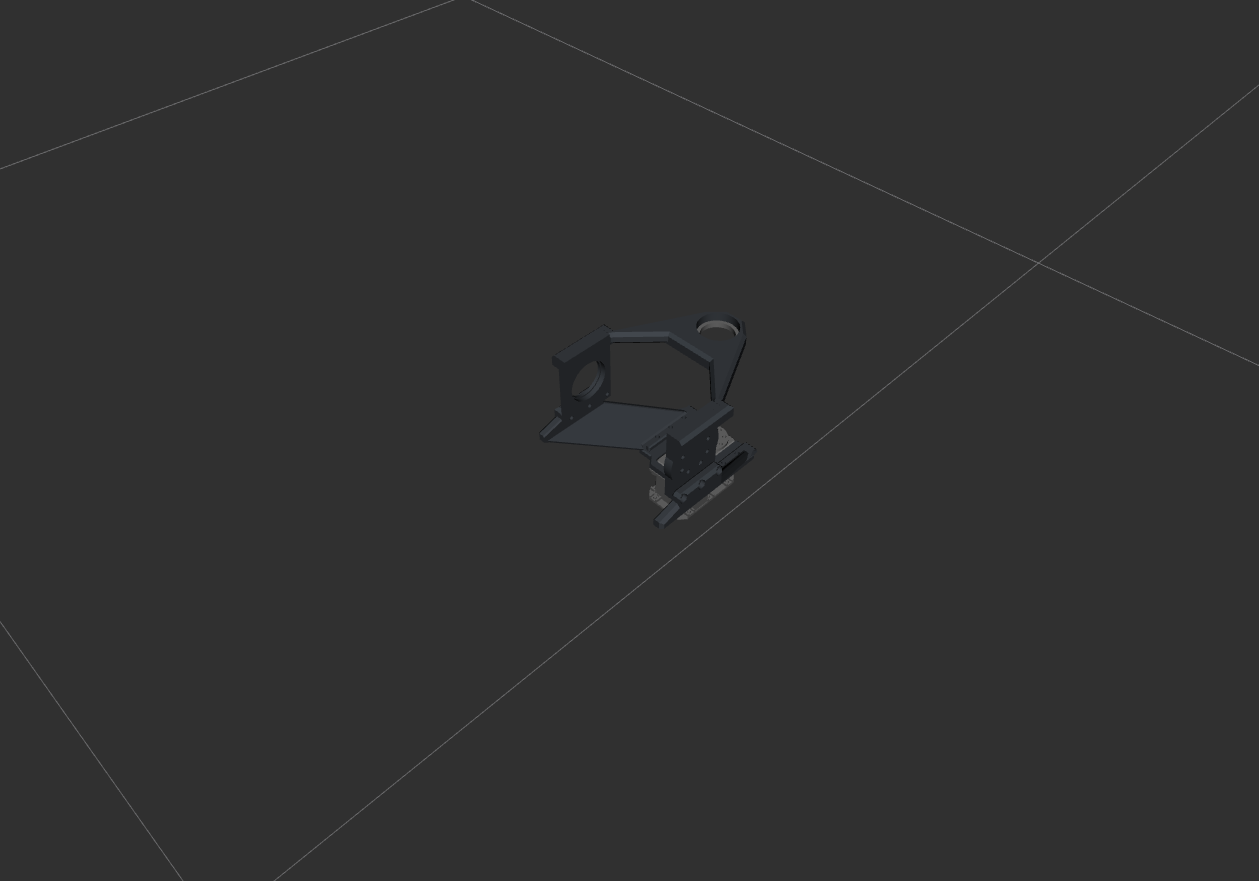
\includegraphics[width=\linewidth]{link3.png}
    \caption{link3}
  \end{subfigure}
  \begin{subfigure}[b]{0.2\linewidth}
    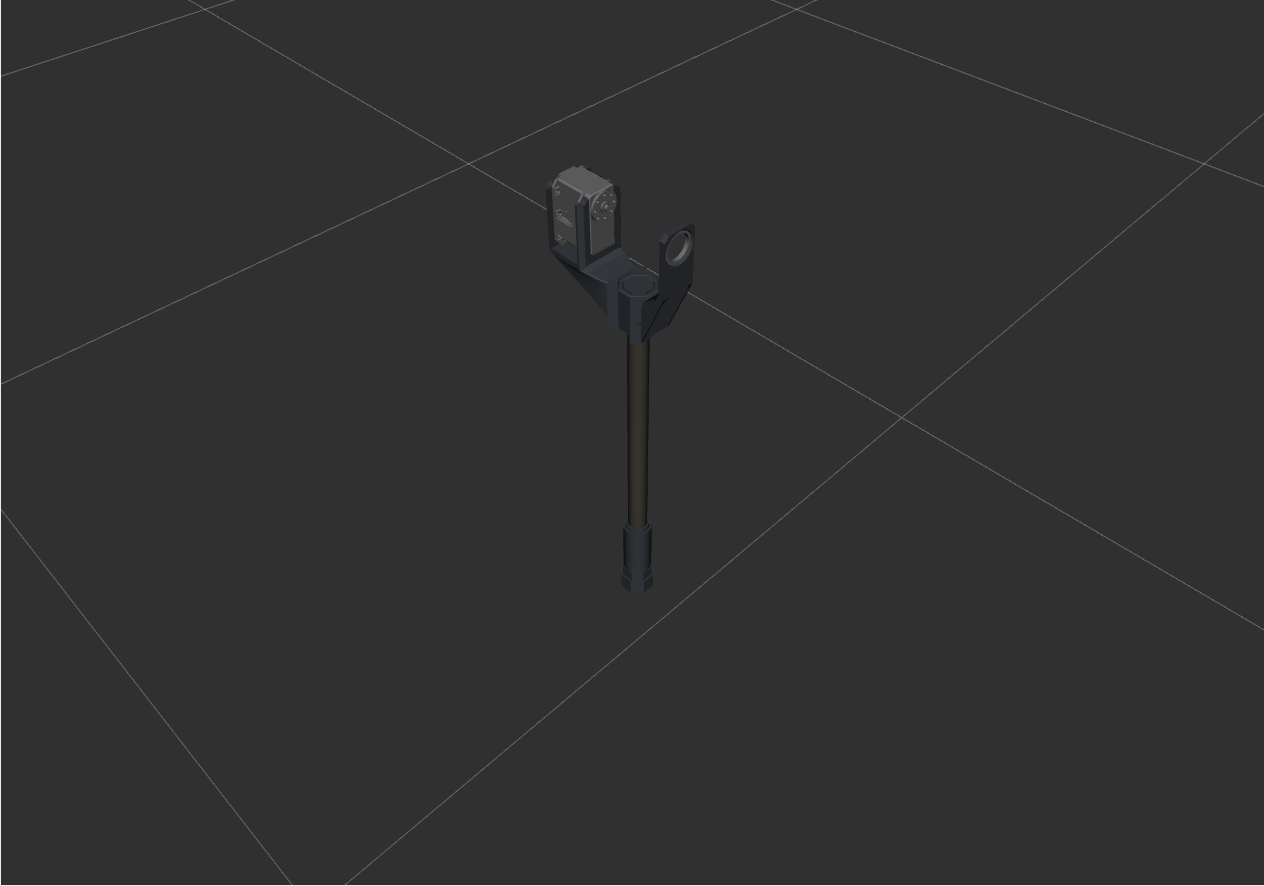
\includegraphics[width=\linewidth]{link4.png}
    \caption{link4}
  \end{subfigure}
  \begin{subfigure}[b]{0.2\linewidth}
    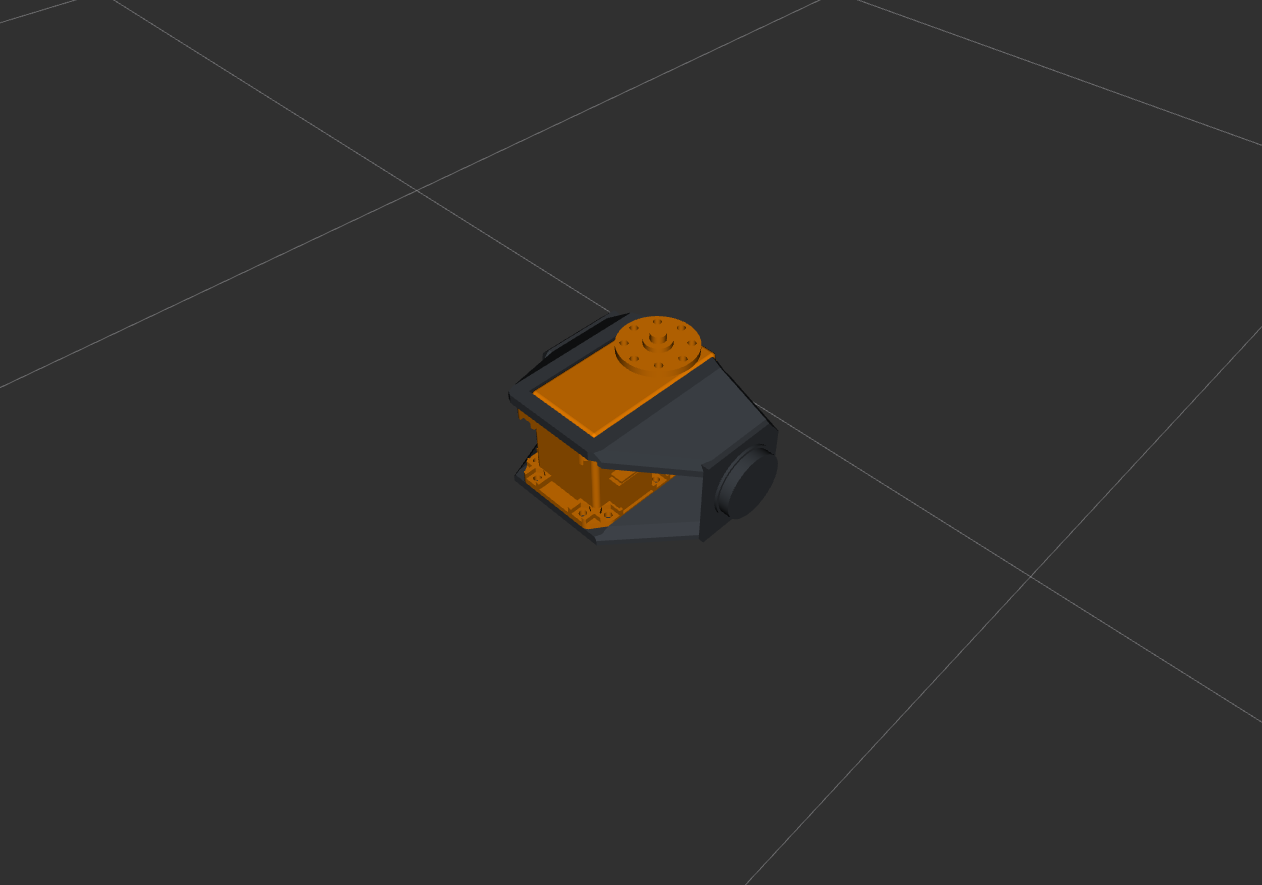
\includegraphics[width=\linewidth]{link5.png}
    \caption{link5}
  \end{subfigure}
  \begin{subfigure}[b]{0.2\linewidth}
    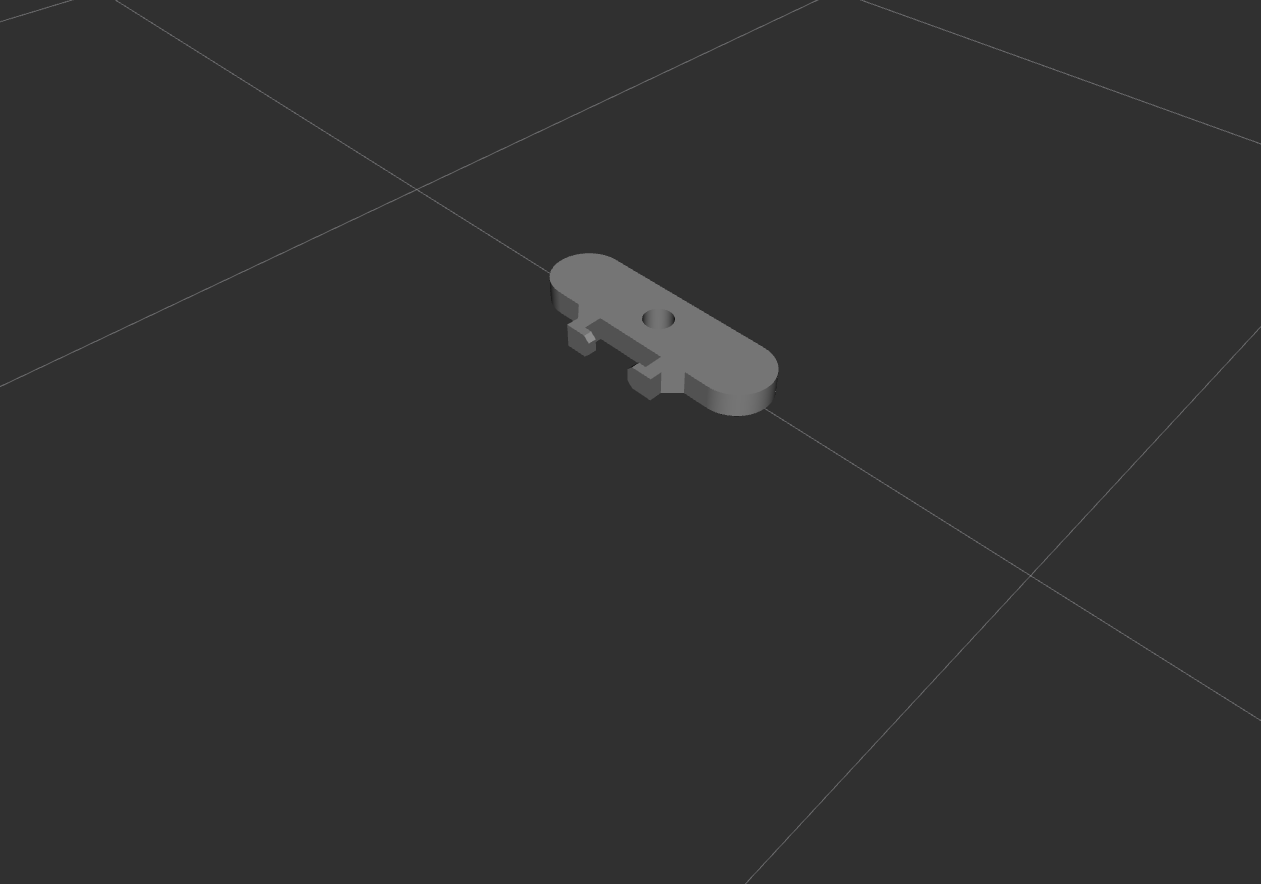
\includegraphics[width=\linewidth]{link6.png}
    \caption{link6.}
  \end{subfigure}
  \begin{subfigure}[c]{0.4\linewidth}
    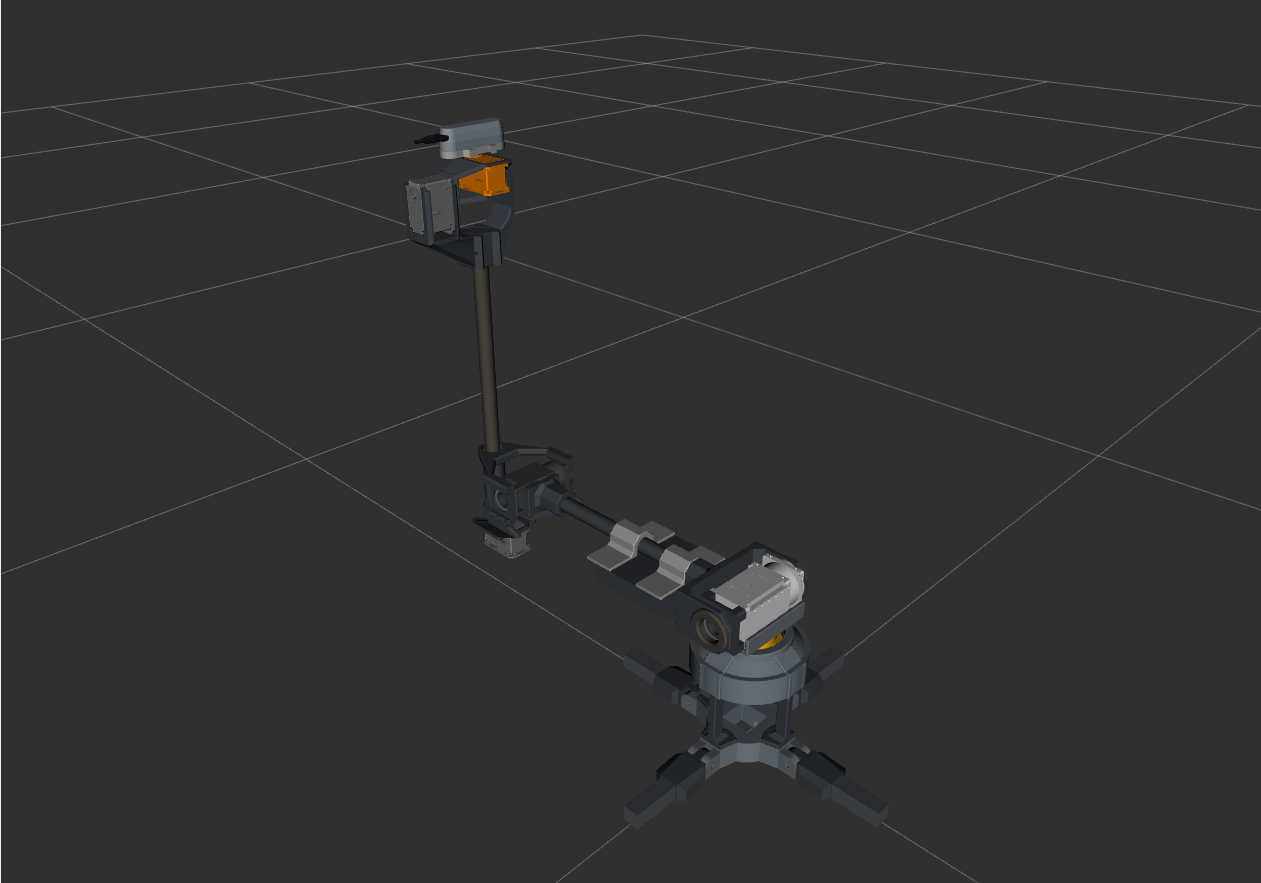
\includegraphics[width=\linewidth]{r_mini.png}
    \caption{Rimini in simulation}
  \end{subfigure}
  \begin{subfigure}[c]{0.4\linewidth}
    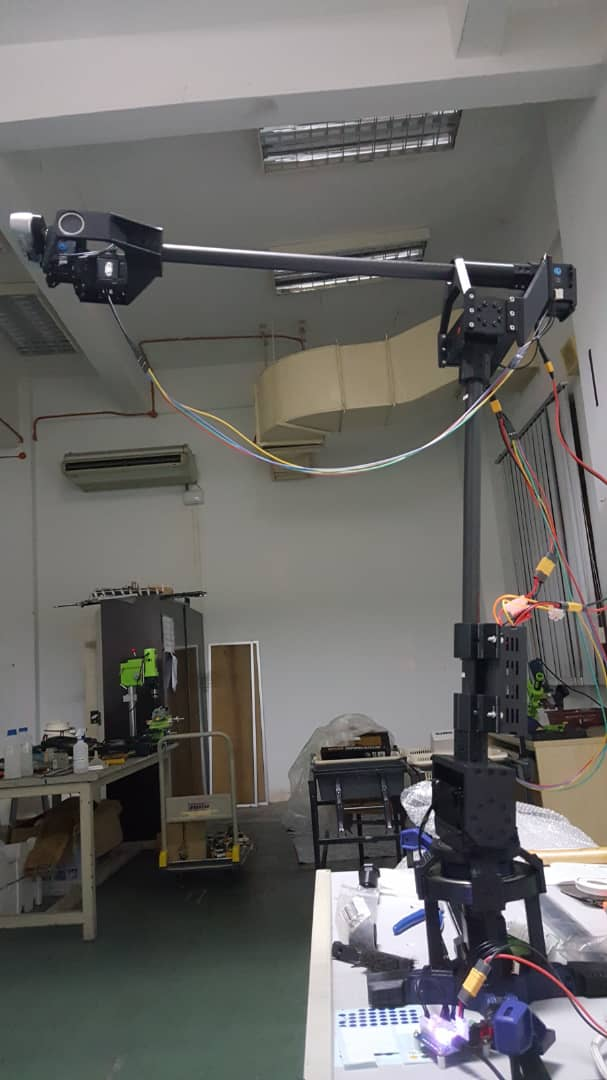
\includegraphics[width=\linewidth]{r_mini_hw.jpeg}
    \caption{Rimini build completion.}
  \end{subfigure}

\caption{Rimini and its links}
  \label{fig:rimini_links}
\end{figure}
